\documentclass{beamer}
\usepackage[utf8]{inputenc}
\usepackage[czech]{babel}
\usepackage{graphicx}
\usepackage{listings}
\usepackage{multicol}
\usepackage{multirow}
\usepackage{algorithm}
\usepackage{algorithmic}
\usepackage{caption}
\usepackage{amsfonts}
\usepackage{amssymb}
\usepackage{amsmath}
\usetheme{Frankfurt}

\title{Shongo}
\subtitle{Reservation system for video and web conferences}
\author{Martin Šrom, Petr Holub, Onřej Pavelka}
\date{November 25, 2013}
\institute{

\includegraphics[width=0.3\textwidth]{cesnet.pdf}
}

% Algorithm
\newcommand{\algf}{\fontsize{2.5mm}{2.5mm}\selectfont}
\newcommand{\algc}[1]{\algf\textbf{#1}}
\algsetup{linenosize=\algf}

% Listings
\lstset{
  basicstyle=\ttfamily\scriptsize,
  keywordstyle=[1]{\textbf},
  morekeywords=[1]{begin,end,if,then,endif},
}

\beamertemplatenavigationsymbolsempty

\begin{document}

\begin{frame}
  \titlepage
\end{frame}

\section{Shongo}\subsection{}
\begin{frame}
  \frametitle{Shongo}
  
  \begin{itemize}
    \item Reservation system for video or web conferencing resources
    \item Performs:
    \begin{itemize}    
      \item \textbf{Booking} -- ensure the availability of resources
      \vspace*{1mm}\newline\textit{Examples:}\vspace*{-0.5mm}
      \begin{itemize}
        \item \textit{guarantee available ports to each virtual room in Cisco MCU}
        \item \textit{reservation of hardware endpoints and/or meeting rooms}
      \end{itemize}\vspace*{1mm}
      \item \textbf{Execution} -- automation of repetitive tasks
      \vspace*{1mm}\newline\textit{Examples:}\vspace*{-0.5mm}
      \begin{itemize}    
        \item \textit{create new virtual room in Adobe Connect }
        \item \textit{dial-in of H.323 hardware endpoint}
        \item \textit{start recording/streaming of virtual room in Cisco MCU}
      \end{itemize}\vspace*{1mm}
      \item \textbf{Management} -- runtime management of resources
      \vspace*{1mm}\newline\textit{Examples:}\vspace*{-0.5mm}
      \begin{itemize}    
        \item \textit{watch device status}
        \item \textit{watch virtual rooms in multipoint devices}
        \item \textit{watch active participants in virtual room}
        \item \textit{change attributes of virtual room and its participants}
      \end{itemize}\vspace*{1mm}
    \end{itemize}
  \end{itemize}          
\end{frame}

\begin{frame}
  \frametitle{Architecture}
  \begin{itemize}
    \item Multi-domain (inter-domain booking protocol)
    \item Each domain:
    \begin{itemize}
      \item \textbf{Controller} -- main backend component with APIs
      \newline\textit{resource database, booking, execution and management}
      \item \textbf{Connectors} -- components acting as “drivers” for devices
      \newline\textit{performs commands in individual devices}
      \item \textbf{Clients} -- used by users and administrators to access controller
      \newline\textit{enables users/administrators to book and manage resources}
    \end{itemize}
  \end{itemize}
  \begin{center}
  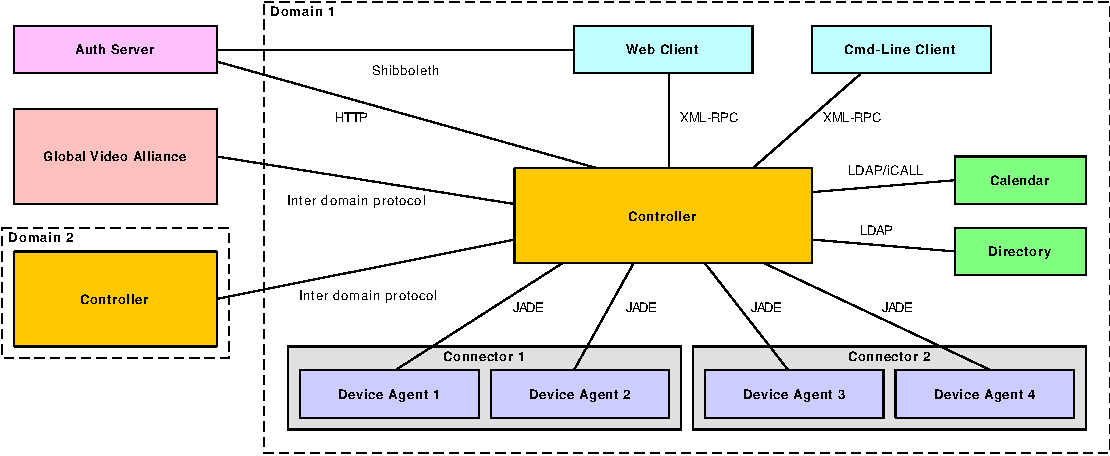
\includegraphics[width=0.9\textwidth]{../architecture/diagrams/dd_architecture.pdf}
  \end{center}
\end{frame}

\begin{frame}
  \frametitle{Current State}
  \begin{itemize}
    \item Standalone domains (without inter-domain protocol)
    \item Connectors:
    \begin{itemize}
      \item Cisco MCU (4200/4500/4500 Series, MSE 8420/8510)
      \item Adobe Connect
      \item Cisco Codec C90, Lifesize (endpoints)
    \end{itemize}
    \item\textbf{Command-Line Client} for administrators
    \newline\textit{to manage Controller}
    \item\textbf{Web Client} for users (and administrators)
    \newline\textit{to book and manage virtual rooms in multipoint devices}
  \end{itemize}
  \begin{center}
  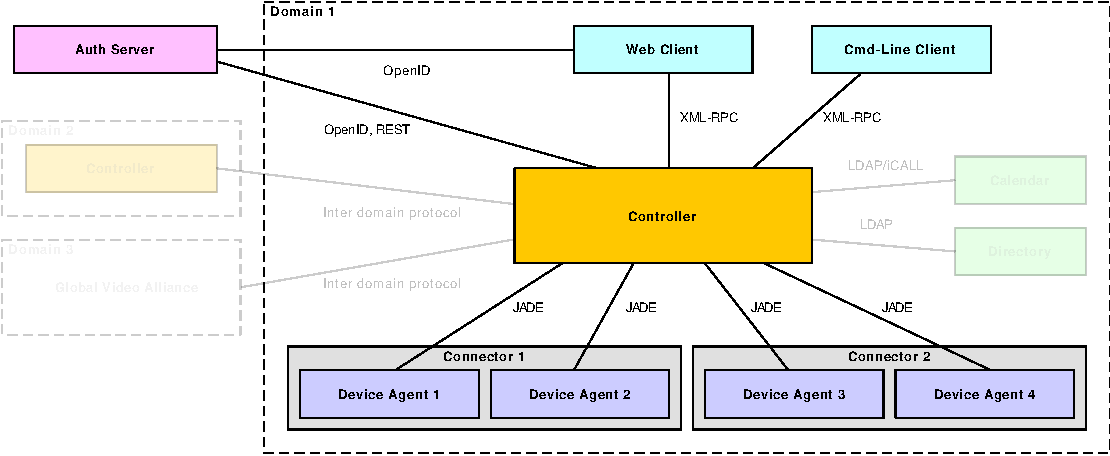
\includegraphics[width=0.8\textwidth]{../architecture/diagrams/dd_architecture_implemented.pdf}
  \end{center}
\end{frame}

\begin{frame}
  \frametitle{Future}
  \begin{itemize}
    \item Recording of virtual rooms (\textit{in development})
    \item Multiple identities per user (\textit{in development})
    \item Streaming of virtual rooms
    \item Adobe Connect seminar rooms
    \item Administrator control panel in web client
    \item Inter-domain booking protocol
  \end{itemize}
\end{frame}

\section{Web Client Demo}\subsection{}

\begin{frame}
  \frametitle{Web Client Demo}
  \begin{itemize}
    \item Log-in
      \begin{itemize}
        \item Hostel registration    
      \end{itemize}
    \item Dashboard
      \begin{itemize}
        \item Time zone and language settings
        \item Create new Ad-hoc room (configuration of participants)
        \item Create new Permanent room (configuration of user roles)
        \item Create capacity for the permanent room (periodicity)
      \end{itemize}
    \item Email notifications      
    \item Room management
      \begin{itemize}
        \item Active participants
      \end{itemize}    
    \item List of reservation requests
    \item Detail of reservation request
      \begin{itemize}
        \item Modify the reservation request
        \item History of the reservation request        
      \end{itemize}          
  \end{itemize}
\end{frame}

\end{document}